\section{Architecture}

This section covers the architecture of the developed sparse linear algebra (Spla for short) library, primary components and modules, the sequence of operations processing on the GPUs. The library is designed in order to overcome the limitation of the existing solutions, mentioned in the previous section.

\subsection{Design principles}

The library is designed the way to maximize potential library performance, simplify its implementation and extensions, and to provided the end-user verbose, but effective interface allowing customization and precise control over operations execution. These ideas are captured in the following principles.

\begin{itemize}
    \item \textbf{Optional acceleration}. Library is designed in a way, that GPU acceleration is fully optional part. Library can perform computations using standard CPU pipeline. If GPU is supported, library can offload a part of a work for accelerator.

    \item \textbf{Manual scheduling}. The user defines tasks for computations in the form of a schedule object. Schedule consists of a series of dependent step. Each step has a list of prioritised independent tasks. The uses assembles schedule using  The user then passes the entire schedule to the library for execution, and can either block or wait in a non-blocking way the result.
    
    \item \textbf{Predefined types}. The library provides the ability to parameterize operations using a set of predefined types. The type is represented by the unique name and size of the elements in bytes. The elements of the type are POD structures, treated as regular byte sequences. Standard types are supported.
    
    \item \textbf{Rich functions set}. The library provides the ability to parameterize operations using predefined functions, declared over supported standard types. Functions are built-in. They have a C++ and OpenCL analogues integrated into library core.  
    
    \item \textbf{Explicit execution}. The library automatically splits the expression graph into many tasks and subtasks, which are ordered according to dependencies and distributed to the GPU device. This work is hidden from the user and does not require any action from him.
    
    \item \textbf{Multiple storage formats}. The library provides a generalized mechanism to store a data in a number of different formats. It is done in a form of decorators. A decorator stores data in a single format. Decorators can be created on demand by different parts of the library. Transformation rules used to synchronize data between decorators.
    
    \item \textbf{Exportable interface}. The library has a C++ interface with an automated reference-counting and with no-templates usage. It can be wrapped by C99 compatible API and exported to other languages, for example, in a form of a Python package.
\end{itemize}

\subsection{Design overview}

The general library design idea is depicted in a figure~\ref{fig:design_idea}. The most import part of the design is that the GPU acceleration is a fully optional part of the library. Thus, the library can function in any environment even without GPU. This design is dictated by the following considerations.

\begin{itemize}
    \item \textbf{CPU and GPU asymmetry}. CPU and GPU are not equal devices for programming and execution. The GPU device is always in a satellite mode relatively to the CPU. CPU defines the control sequence for a GPU. CPU and GPU also capable of doing a bit different things. Thus, CPU must remain the main part of the design library in order to reflect this peculiarities. 
    \item \textbf{GPU complexity}. GPU is a very complex thing to program. GPU requires additional algorithms and data structures to work properly. Thus, this complexity must be isolated in a form of fully optional module.
    \item \textbf{GPU specifics}. GPU has specialized requirements for data allocation and layout. Thus, CPU data must be duplicated, transformed and processed into specialized acceleration structures, stored on a GPU. It introduces duplication of data. But, it can be neglected. RAM has order of magnitude bigger size then the bleeding edge VRAM of a modern video card.
    \item \textbf{User experience}. Data analysis involves a lot of tasks. Not all tasks can be leveraged to GPU. It involves complex data processing, statics, read queries, etc. Thus, some work must be done on a CPU.
    \item \textbf{Modularity}. Modular design allows replacement of computations accelerators on fly. Thus, it can be possible to use multi-core CPUs, different GPUs APIs, and even multi-GPUs as acceleration backends without any existing code modifications.
\end{itemize}

\begin{figure}[ht]
    \centering
    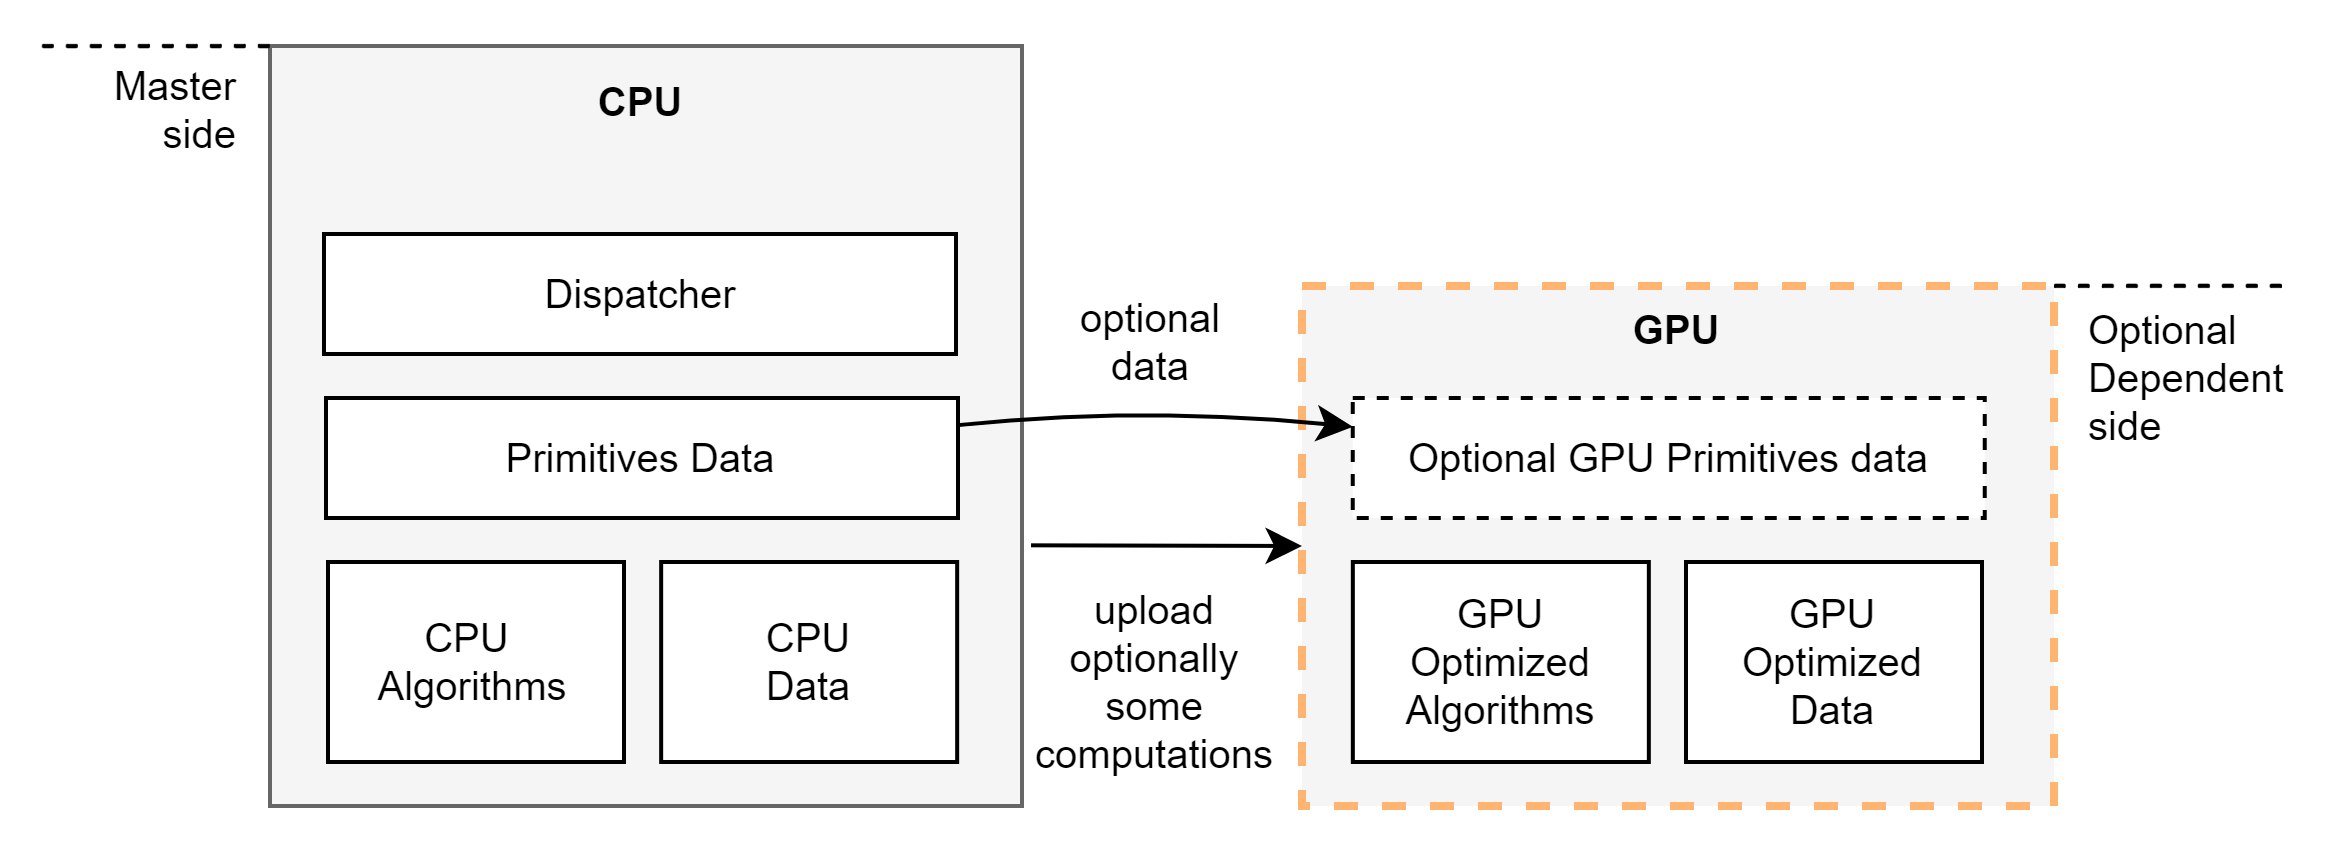
\includegraphics[width=1.0\textwidth]{images/spla_design_idea.png}
    \caption{Library primary design idea. The CPU side of the library is a master. It is fully featured to perform computations. GPU is an optional acceleration. It can be used to offload some work. Data and algorithms support is optional.}
    \label{fig:design_idea}
\end{figure}

\subsection{Execution model}

The general idea of the library schedule execution is depicted in the figure~\ref{fig:execution_schema}.

As an input library accepts the expression in a form of a schedule. The schedule is created using library API. The schedule is built from a number of a sequential steps. Steps are ordered. The next step starts only when the previous step is fully finished. Each step is composed from a sorted by a priority list of tasks. Single task represents and fundamental operation, which processes matrices or vectors. This operation can be product, assignment, transposition, etc. Tasks will be started independently in the order, defined by priorities. 

Number of parallel tasks can be limited by a number of factors. Number of available CPU threads as well as number of GPU queues defines how many tasks run in parallel. GPU has a limited number of hardware queues for submitting commands. In most cases it is limited up to only a single queue. Thus, on some GPUs it is not possible to get any parallelism from parallel tasks.  

\begin{figure}[ht]
    \centering
    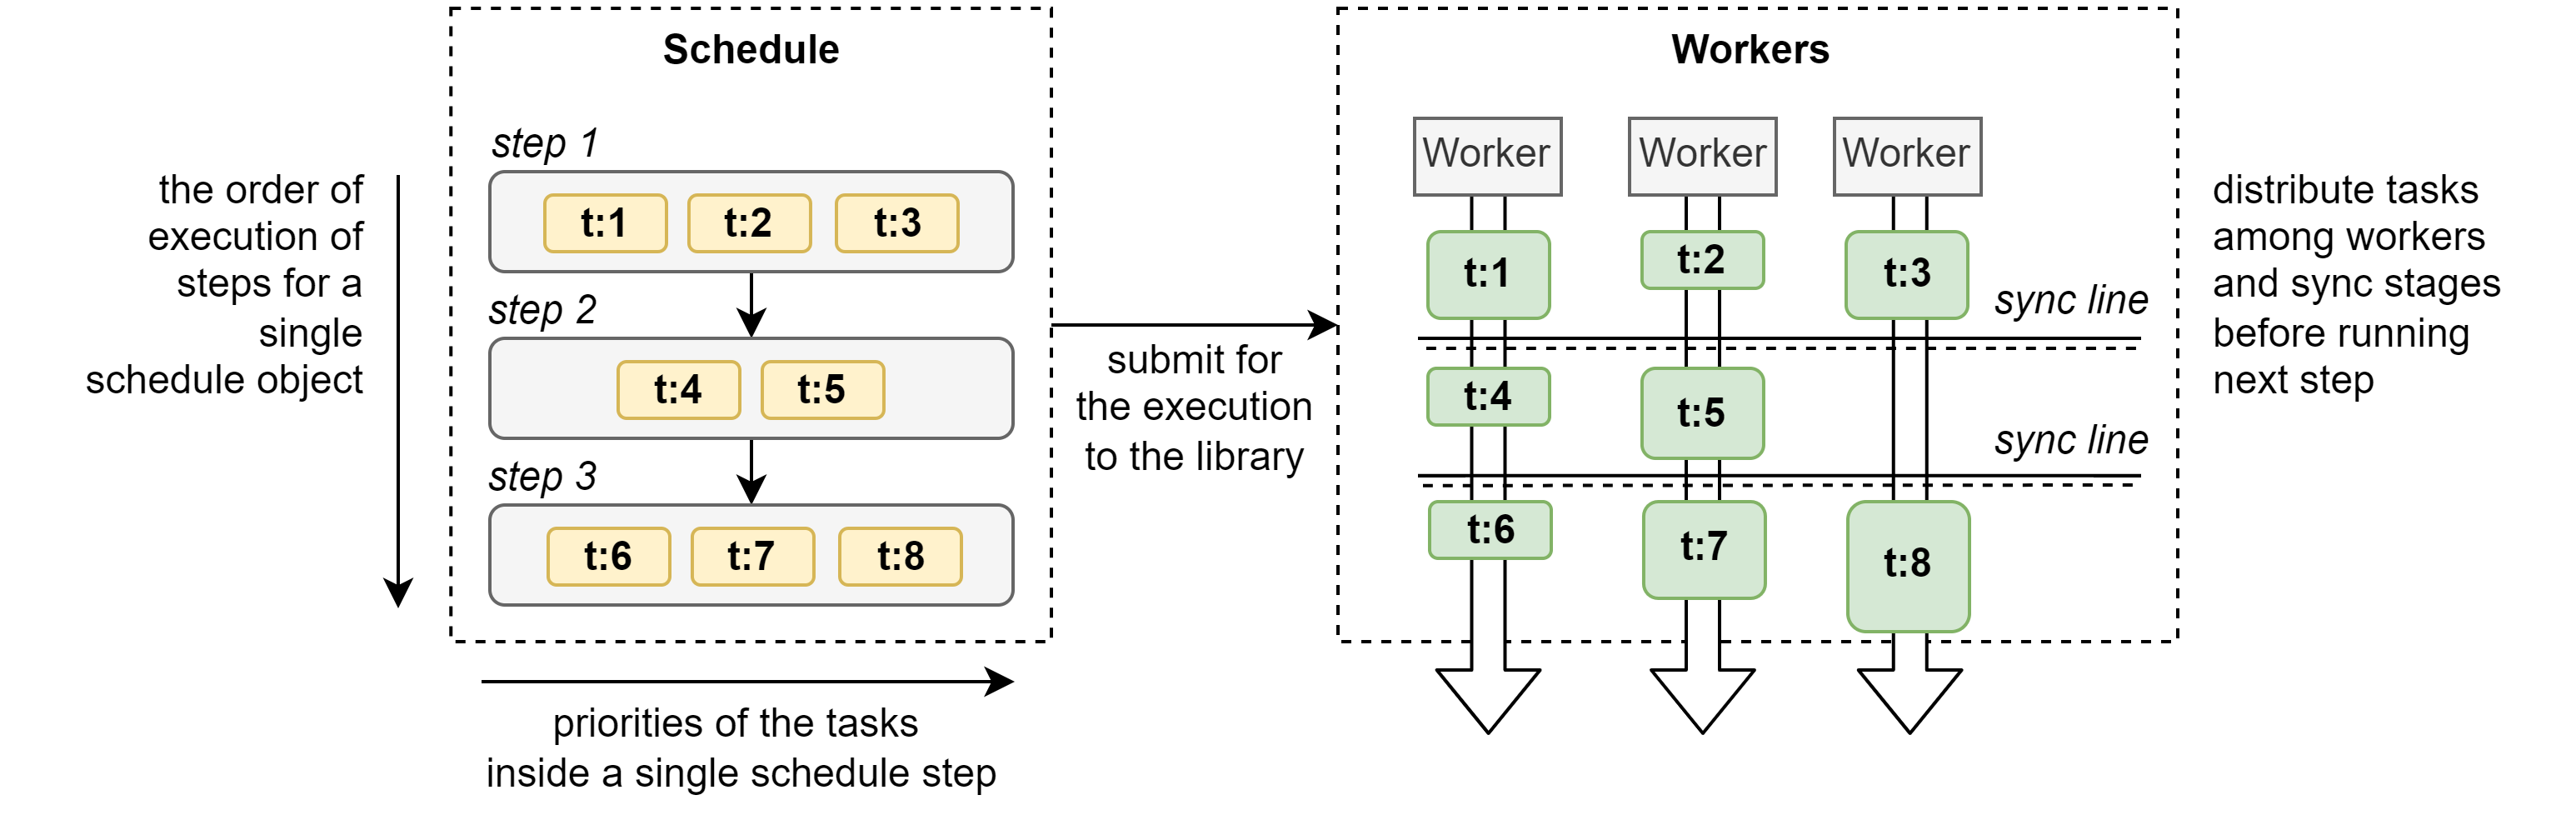
\includegraphics[width=1.0\textwidth]{images/spla_scheduling.png}
    \caption{Library schedule execution idea.}
    \label{fig:execution_schema}
\end{figure}

The schedule is submitted to the library for the execution. The schedule is traversed and for each task in a step the algorithm for execution is found. The algorithm is responsible for a processing of a single task. It is possible to have multiple task for a single type operations with specialized rules of selection. This approach allows to separate the data and the execution, as well as gives an ability to handle some edge cases and optimize operation for a particular set of input arguments.

Each algorithm is responsible for the evaluation of a single task. Task is passed as an argument. Algorithm obtains all necessary parameters through the task using runtime type system.

Schedules are executed asynchronously. The user after submission gets a special \textit{future} object, which allows either to block until completion or to probe the state of the schedule in a non-blocking fashion.

For the sake of simplicity, each operation can be run in an procedural fashion without a schedule. In this case, dummy schedule is constructed under the hood, submitted and immediately executed. It is convenient for simple user algorithms without complex scheduling potential.

\subsection{Data Storage}

Library provides flexible and extensible hybrid decorations' based storage format. The idea of the storage is depicted in a figure~\ref{fig:vec_storage}. This storage model aims to solve the following problems.

\begin{figure}
    \centering
    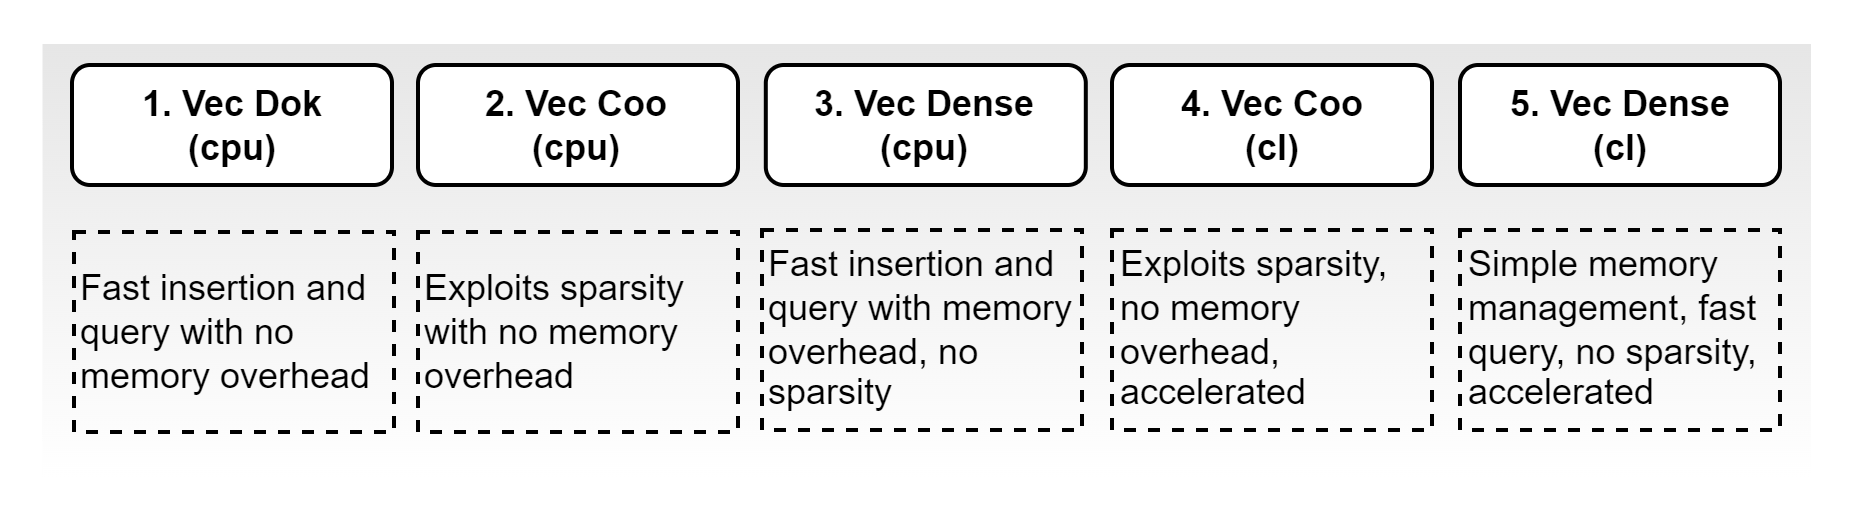
\includegraphics[width=1.0\textwidth]{images/spla_vector_storage.png}
    \caption{Vector decorations storage. Storage provides slots for different representations. Representation choice depends on a task currently being solved.}
    \label{fig:vec_storage}
\end{figure}

\begin{itemize}
    \item \textbf{Format flexibility}. There is no the silver bullet storage for allow tasks. Thus, different formats must be employed for distinct tasks solving. What is more important if we talking about GPUs acceleration. GPU has distinct memory space and unique memory layout requirements. Also, layout of the data may vary depending on type of operations, which reads, modifies, or entirely updates the content of the vector or matrix on a GPU. 

    \item \textbf{Data synchronization}. The presence of multiple valid decorations with vector or matrix data causes data transformations. Thus, data for one target decoration can be actualized from another source decoration. This data transformation must be formalize in terms of different rules, so it is possible add new formats to the storage.

    \item \textbf{Code complexity}. Formalization of storage mechanism in a form of programmable set of rules is required. The complexity of convertation has quadratic nature if we want to support N different storage formats. Thus, formalization must be don prior to standardize the way of how new format is added to the library. 

    \item \textbf{Generalization}. This storage mechanism can be used for both vector and matrix storage. It makes it usable and very powerful thing. Potentially, it allows adding new primitives to the library reusing existing storage schema. Decorations can be create to hold any data useful for the application.

    \item \textbf{Interoperability}. Library storage schema also must solve the interoperability issues. Decorations can hold any data. It allows to support NumPy and Sci-Py based primitives without modification of any existing source code.
\end{itemize}

The idea of storage transformation graph is depicted in a figure~\ref{fig:vec_storage_graph}. Transformations graph defined using rules as oriented edges between formats. The presence of an arrows shows, that here is a rule to convert one decorator data into other decorator data. These rules can be used to synchronize decorations data on demand. 

\begin{figure}
    \centering
    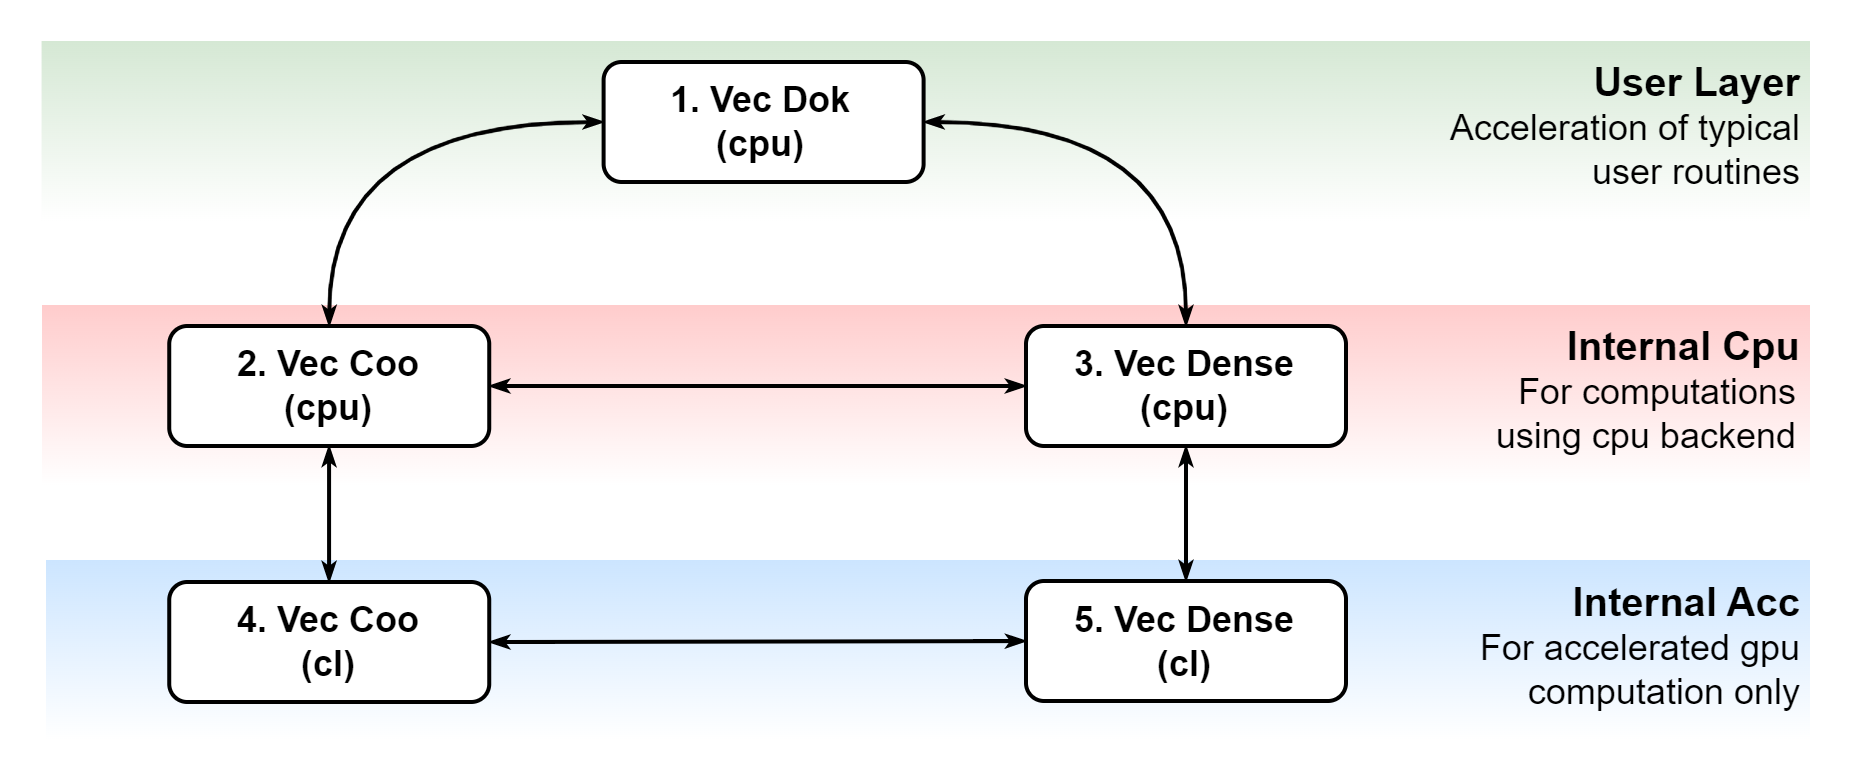
\includegraphics[width=1.0\textwidth]{images/spla_storage_transformation_graph.png}
    \caption{Vector decorations storage transformations graph. Graph declares transformation rules between different decoration formats. Existence of a path in this graph allows to convert one decoration into another automatically.}
    \label{fig:vec_storage_graph}
\end{figure}

For an instance, consider a task of obtaining a decoration in a dictionary of keys (dok cpu) format for user read operations in figure~\ref{fig:vec_transform_path}. The storage keeps tracking of valid decorations with valid data. In our example currently valid decoration is list of coordinates decoration for OpenCL device (vec coo cl). The transformation graph searches for the shortest path between node 4 and 1 in a rules graph. Then it issues conversations. The first convertation will copy OpenCL data to CPU data into vector list of coordinates for CPU side. Then, this data will be converted further into a dictionary of keys. After that, the data stored on GPU can be used as a dok on a CPU for fast queries and modifications.

\begin{figure}
    \centering
    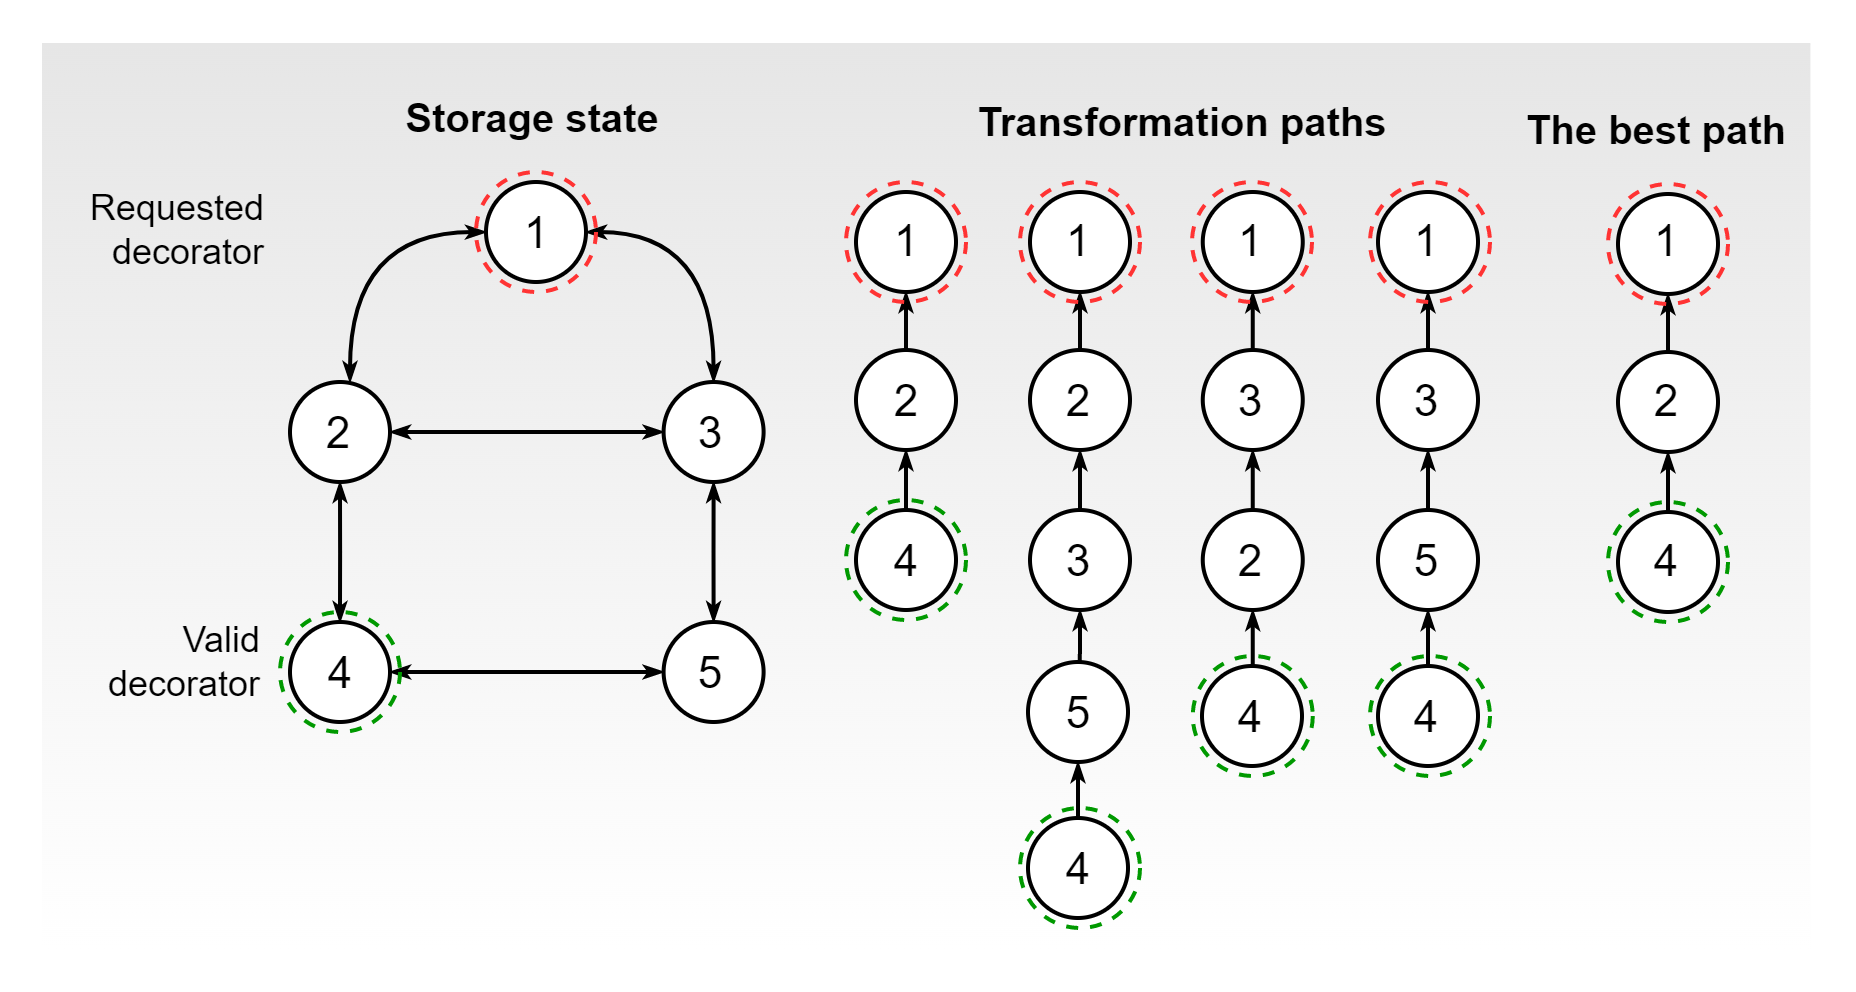
\includegraphics[width=1.0\textwidth]{images/spla_storage_transformation.png}
    \caption{Vector storage transformation process. Target format is 1 (red circle). Source format is 4 (green circle). The shortest path is the best path for convertation.}
    \label{fig:vec_transform_path}
\end{figure}

The transformation process might be costly. It can involve several transformation stages. Also, its complexity depends on the amount of data to convert. Thus, the transformation must be avoided as much as it can. In this case, typical strategy for a data processing is following. 

\begin{itemize}
    \item User uploads all the necessary data into matrices and vectors.
    \item User issues a preparation the data. Internally it will be converted into suitable formats.
    \item Then user performs and number of computations states keeping data on the accelerator side without unnecessary read-backs.
    \item Finally, user copies result of the computations back to the CPU to analyse achieved results.
\end{itemize}

\subsection{Algorithms registry}

This section describes how different algorithms implementations stored in the library how it is found on a request. Algorithms registry aims to solve the following tasks.

\begin{itemize}
    \item Registry segregates algorithms declarations and its particular invocations. It allows to dispatch algorithms dynamically at runtime what gives flexibility for a configuration.
    \item Registry allows to query for supported and not supported algorithm. It gives an ability to select algorithm at runtime. If algorithm is not presented, then we can fallback to other less optimized version.
    \item Registry gives an ability to store multiple versions of the same algorithm for different platforms and accelerations backends.
\end{itemize}

Idea of the registry storage is shown in a figure~\ref{fig:algo_registry}. Registry is a key value storage like a dictionary. As a key strings with special formatting are employed. This strings are constructed from an operation description which must be evaluated. Dispatcher appends the suffix of a target device or backend for computations. If key is presented, then the algorithm is used. Otherwise some fallback implementation is utilized.

\begin{figure}
    \centering
    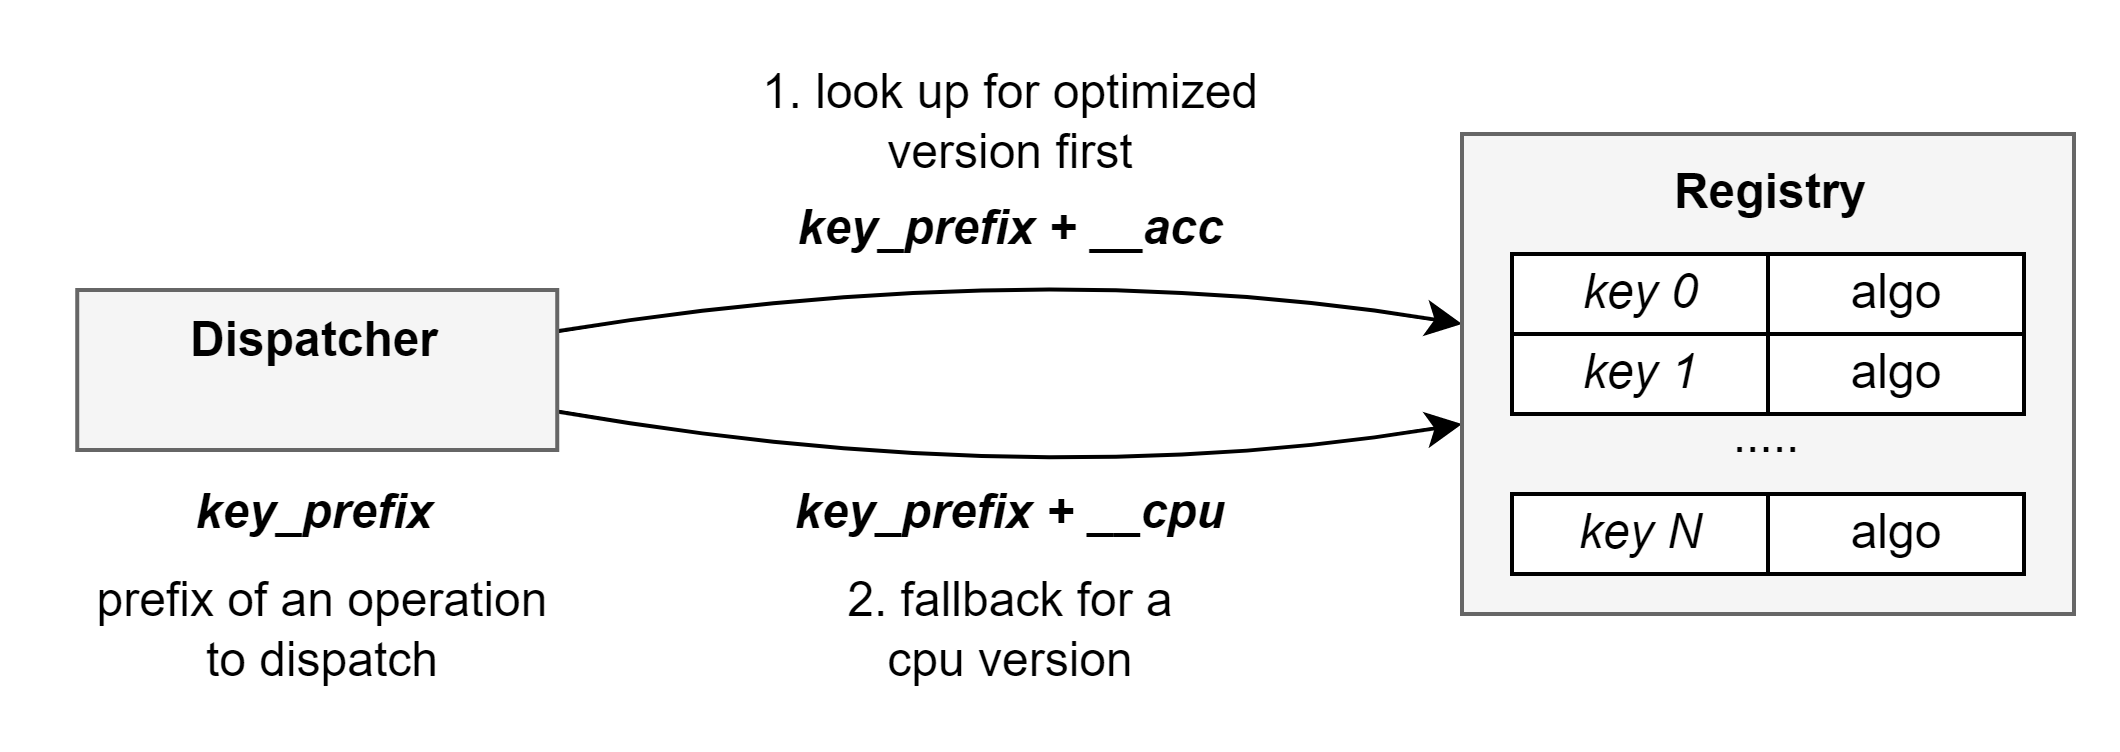
\includegraphics[width=1.0\textwidth]{images/spla_algo_registry.png}
    \caption{Registry of algorithms. Dispatcher looks up for optimized algorithms first. As a fallback it uses cpu suffix to get default algorithm implementation without an acceleration.}
    \label{fig:algo_registry}
\end{figure}

The structure of keys is depicted in a figure~\ref{fig:algo_key}. The key is effectively a string literal, which is constructed using specialized rules. The prefix of the key is the name of the operation which must be evaluated. As a name for operation actual mathematical name can be used, such as matrix-vector product, matrix-matrix product, etc. 

The name is followed by the name of used functions and their type codes. Mathematical functions must be parameterized by scalar functions. Each function has a name and a set of type codes for each type of the argument. Scalar multiplication and addition functions has three opcodes. Since each function is a binary operator of type $A \times B \xrightarrow{} C$. 

Binary functions are followed by a selection operation. Selection is an unary function with the signature $A \xrightarrow{} bool$. Selection operator is used to filter final results using masking. Typically, we are not interested in a whole result. So the mask is provided. Type of mask values used to parameterize select operation. Selection can be any unary predicate. In most cases, greater than, equals or not equals zero are the most used one.

Finally, the key prefix is appended with a code of a backend  for computations. Different accelerators, including cpu fallback, may be supported for computations. Using accelerator suffix allows to switch between backend at runtime and select the most optimized algorithm. 

It is possible that there is no algorithms for a given key. Thus, the fallback version must be utilized. In order to do that, key prefix may be concatenated with a cpu suffix. All algorithms have a cpu analogues in a registry.

Keys in a form of a string solve two major problems. Firstly, it gives a readable and human understandable representation of an operation. Secondly, it allows to actually segregate an operation with its arguments and particular algorithm instance. Algorithm is an object with its own state and unified interface. It allows to maximize the performance and reuse artifacts, which may appear between algorithm invocations, such as GPU kernels, acceleration structures, etc. 

\begin{figure}[]
    \centering
    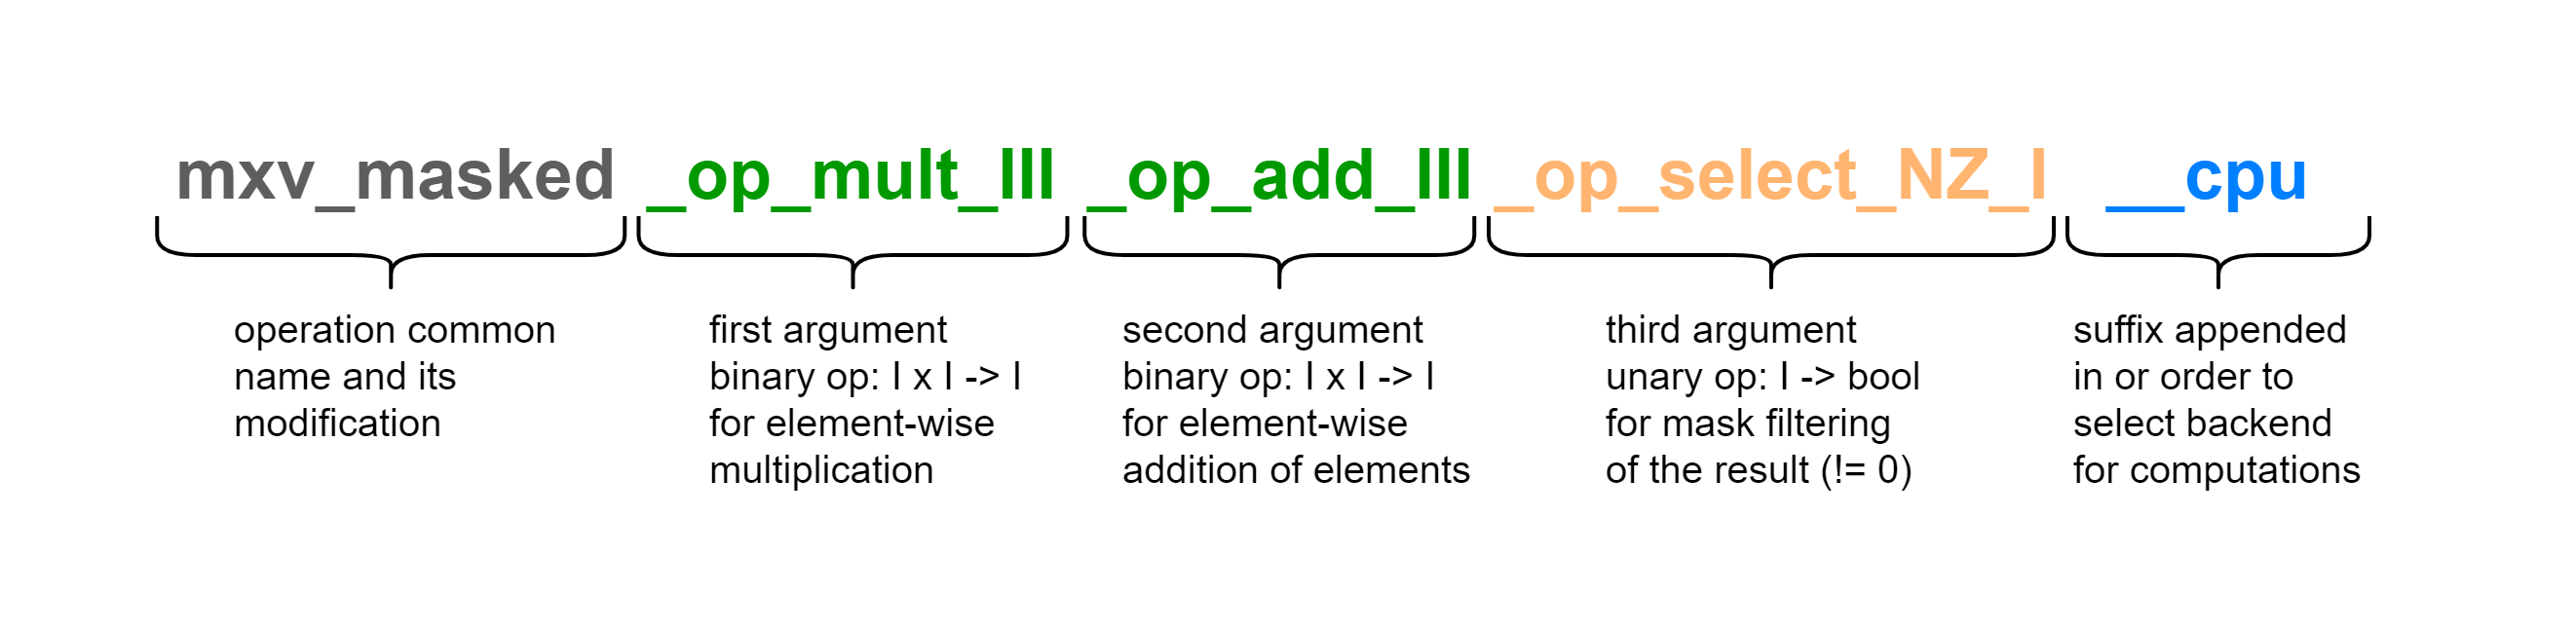
\includegraphics[width=1.0\textwidth]{images/spla_algo_key.png}
    \caption{The structure of an algorithm key. The is a string literal composed from several parts. Prefix shows the algorithm name and its parametrization by operations. The suffix of the key shows which backed or accelerator to use for the evaluation of the algorithm.}
    \label{fig:algo_key}
\end{figure}